
%%--------------------------------------------------
%% Serway: Physics for Scientists and Engineers
%%--------------------------------------------------


%% Chapter 07: Energy and Energy Transfer
%%--------------------------------------------------


%% Table of Contents
%%--------------------------------------------------

%% 7.1 Systems and Environments 
%% 7.2 Work Done by a Constant Force
%% 7.3 The Scalar Product of Two Vectors
%% 7.4 Work Done by a Varying Force 
%% 7.5 Kinetic Energy and the Work–Kinetic Energy Theorem
%% 7.6 Potential Energy of a System
%% 7.7 Conservative and Nonconservative Forces
%% 7.8 Relationship Between Conservative Forces and Potential Energy
%% 7.9 Energy Diagrams and Equilibrium of a System


%% Serway Multiple Choice Questions
%%--------------------------------------------------
\element{serway-mc}{
\begin{question}{serway-ch07-q01}
    A constant force of \SI{12}{\newton} in the positive $x$ direction acts on a \SI{4.0}{\kilo\gram} object as it moves from the origin to the point $(6\hat{\imath}-8\hat{\jmath})\,\si{\meter}$. 
    How much work is done by the given force during this displacement?
    \begin{multicols}{3}
    \begin{choices}
        \wrongchoice{\SI{+60}{\joule}}
        \wrongchoice{\SI{+84}{\joule}}
      \correctchoice{\SI{+72}{\joule}}
        \wrongchoice{\SI{+48}{\joule}}
        \wrongchoice{\SI{+57}{\joule}}
    \end{choices}
    \end{multicols}
\end{question}
}

\element{serway-mc}{
\begin{question}{serway-ch07-q02}
    A \SI{5.0}{\kilo\gram} object is pulled along a horizontal surface at a constant speed by a \SI{15}{\newton} force acting \ang{20} above the horizontal. 
    How much work is done by this force as the object moves \SI{6.0}{\meter}?
    \begin{multicols}{3}
    \begin{choices}
        \wrongchoice{\SI{78}{\joule}}
        \wrongchoice{\SI{82}{\joule}}
      \correctchoice{\SI{85}{\joule}}
        \wrongchoice{\SI{74}{\joule}}
        \wrongchoice{\SI{43}{\joule}}
    \end{choices}
    \end{multicols}
\end{question}
}

\element{serway-mc}{
\begin{question}{serway-ch07-q03}
    A \SI{2.0}{\kilo\gram} projectile moves from its initial position to a point that is displaced \SI{20}{\meter} horizontally and \SI{15}{\meter} above its initial position. 
    How much work is done by the gravitational force on the projectile?
    \begin{multicols}{3}
    \begin{choices}
        \wrongchoice{\SI{+0.29}{\kilo\joule}}
      \correctchoice{\SI{-0.29}{\kilo\joule}}
        \wrongchoice{\SI{+30}{\joule}}
        \wrongchoice{\SI{-30}{\joule}}
        \wrongchoice{\SI{-50}{\joule}}
    \end{choices}
    \end{multicols}
\end{question}
}

\element{serway-mc}{
\begin{question}{serway-ch07-q04}
    How much work is done by a person lifting a \SI{2.0}{\kilo\gram} object from the bottom of a well at a constant speed of \SI{2.0}{\meter\per\second} for \SI{5.0}{\second}?
    \begin{multicols}{3}
    \begin{choices}
        \wrongchoice{\SI{0.22}{\kilo\joule}}
      \correctchoice{\SI{0.20}{\kilo\joule}}
        \wrongchoice{\SI{0.24}{\kilo\joule}}
        \wrongchoice{\SI{0.27}{\kilo\joule}}
        \wrongchoice{\SI{0.31}{\kilo\joule}}
    \end{choices}
    \end{multicols}
\end{question}
}

\element{serway-mc}{
\begin{question}{serway-ch07-q05}
    A \SI{2.5}{\kilo\gram} object falls vertically downward in a viscous medium at a constant speed of \SI{2.5}{\meter\per\second}. 
    How much work is done by the force the viscous medium exerts on the object as it falls \SI{80}{\centi\meter}?
    \begin{multicols}{3}
    \begin{choices}
        \wrongchoice{\SI{+2.0}{\joule}}
        \wrongchoice{\SI{+20}{\joule}}
        \wrongchoice{\SI{-2.0}{\joule}}
      \correctchoice{\SI{-20}{\joule}}
        \wrongchoice{\SI{+40}{\joule}}
    \end{choices}
    \end{multicols}
\end{question}
}

\element{serway-mc}{
\begin{question}{serway-ch07-q06}
    A \SI{2.0}{\kilo\gram} particle has an initial velocity of $(5\hat{\imath}-4\hat{\jmath})\,\si{\meter\per\second}$.
    Some time later, its velocity is $(7\hat{\imath}+3\hat{\jmath})\,\si{\meter\per\second}$.
    How much work was done by the resultant force during this time interval,
        assuming no energy is lost in the process?
    \begin{multicols}{3}
    \begin{choices}
      \correctchoice{\SI{17}{\joule}}
        \wrongchoice{\SI{49}{\joule}}
        \wrongchoice{\SI{19}{\joule}}
        \wrongchoice{\SI{53}{\joule}}
        \wrongchoice{\SI{27}{\joule}}
    \end{choices}
    \end{multicols}
\end{question}
}

\element{serway-mc}{
\begin{question}{serway-ch07-q07}
    A block is pushed across a rough horizontal surface from point $A$ to point $B$ by a force (magnitude $P=\SI{5.4}{\newton}$) as shown in the figure. 
    \begin{center}
    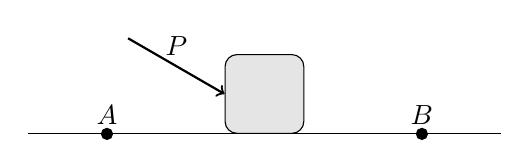
\begin{tikzpicture}
        %% Floor
        \draw (-3,0) -- (3,0);
        \draw[fill] (-2,0) circle (2pt) node[anchor=south] {$A$};
        \draw[fill] (+2,0) circle (2pt) node[anchor=south] {$B$};
        %% Mass
        \node[draw,fill=white!90!black,rectangle,rounded corners=1ex,minimum size=1cm,anchor=south] (A) at (0,0) {};
        %% Force
        \draw[thick,<-] (A.west) -- ++(150:1.414) node[pos=0.5,anchor=south] {$P$};
    \end{tikzpicture}
    \end{center}
    The magnitude of the force of friction acting on the block between $A$ and $B$ is \SI{1.2}{\newton} and points $A$ and $B$ are \SI{0.5}{\meter} apart. 
    If the kinetic energies of the block at $A$ and $B$ are \SI{4.0}{\joule} and \SI{5.6}{\joule}, respectively,
        how much work is done on the block by the force P between $A$ and $B$?
    \begin{multicols}{3}
    \begin{choices}
        \wrongchoice{\SI{2.7}{\joule}}
        \wrongchoice{\SI{1.0}{\joule}}
      \correctchoice{\SI{2.2}{\joule}}
        \wrongchoice{\SI{1.6}{\joule}}
        \wrongchoice{\SI{3.2}{\joule}}
    \end{choices}
    \end{multicols}
\end{question}
}

\element{serway-mc}{
\begin{question}{serway-ch07-q08}
    A constant force of \SI{15}{\newton} in the negative $y$ direction
        acts on a particle as it moves from the origin to the point
        $(3\hat{\imath}+3\hat{\jmath}-1\hat{k})\,\si{\meter}$.
    How much work is done by the given force during this displacement?
    \begin{multicols}{3}
    \begin{choices}
        \wrongchoice{\SI{+45}{\joule}}
      \correctchoice{\SI{-45}{\joule}}
        \wrongchoice{\SI{+30}{\joule}}
        \wrongchoice{\SI{-30}{\joule}}
        \wrongchoice{\SI{+75}{\joule}}
    \end{choices}
    \end{multicols}
\end{question}
}

\element{serway-mc}{
\begin{question}{serway-ch07-q09}
    An object moving along the $x$ axis is acted upon by a force $F_x$ that varies with position as shown. 
    \begin{center}
    \begin{tikzpicture}
        \begin{axis}[
            axis y line=left,
            axis x line=middle,
            axis line style={->},
            xlabel={$x$},
            x unit=\si{\meter},
            xtick={0,2,4,6,8,10,12},
            ylabel={$F_x$},
            y unit=\si{\newton},
            ytick={-10,0,10,20},
            grid=major,
            xmin=0,xmax=12,
            ymin=-12,ymax=22,
            width=0.95\columnwidth,
            height=0.50\columnwidth,
        ]
        \addplot[line width=1pt,mark=\empty] coordinates { (0,20) (2,20) (8,-10) (12,-10) };
        \end{axis}
    \end{tikzpicture}
    \end{center}
    How much work is done by this force as the object moves from $x=\SI{2}{\meter}$ to $x=\SI{8}{\meter}$?
    \begin{multicols}{3}
    \begin{choices}
        \wrongchoice{\SI{-10}{\joule}}
        \wrongchoice{\SI{+10}{\joule}}
      \correctchoice{\SI{+30}{\joule}}
        \wrongchoice{\SI{-30}{\joule}}
        \wrongchoice{\SI{+40}{\joule}}
    \end{choices}
    \end{multicols}
\end{question}
}

\element{serway-mc}{
\begin{question}{serway-ch07-q10}
    A body moving along the $x$ axis is acted upon by a force $F_x$ that varies with $x$ as shown. 
    \begin{center}
    \begin{tikzpicture}
        \begin{axis}[
            axis y line=left,
            axis x line=middle,
            axis line style={->},
            xlabel={$x$},
            x unit=\si{\meter},
            xtick={0,2,4,6,8},
            ylabel={$F_x$},
            y unit=\si{\newton},
            ytick={-8,-4,0,4},
            grid=major,
            xmin=0,xmax=9,
            ymin=-9,ymax=5,
            width=0.95\columnwidth,
            height=0.50\columnwidth,
        ]
        \addplot[line width=1pt,mark=\empty] coordinates { (0,-8) (4,-8) (7,4) (9,4) };
        \end{axis}
    \end{tikzpicture}
    \end{center}
    How much work is done by this force as the object moves from $x=\SI{1}{\meter}$ to $x=\SI{8}{\meter}$?
    \begin{multicols}{3}
    \begin{choices}
        \wrongchoice{\SI{-2}{\joule}}
        \wrongchoice{\SI{-18}{\joule}}
        \wrongchoice{\SI{-10}{\joule}}
      \correctchoice{\SI{-26}{\joule}}
        \wrongchoice{\SI{+18}{\joule}}
    \end{choices}
    \end{multicols}
\end{question}
}

\element{serway-mc}{
\begin{question}{serway-ch07-q11}
    A force acting on an object moving along the $x$ axis is given by
    \begin{equation*}
        F_x = \left(14x-3.0x^2\right)\,\si{\newton}
    \end{equation*}
    where $x$ is in meters. 
    How much work is done by this force as the object moves from $x=\SI{-1}{\meter}$ to $x=\SI{+2}{\meter}$?
    \begin{multicols}{3}
    \begin{choices}
      \correctchoice{\SI{+12}{\joule}}
        \wrongchoice{\SI{+28}{\joule}}
        \wrongchoice{\SI{+40}{\joule}}
        \wrongchoice{\SI{+42}{\joule}}
        \wrongchoice{\SI{-28}{\joule}}
    \end{choices}
    \end{multicols}
\end{question}
}

\element{serway-mc}{
\begin{question}{serway-ch07-q12}
    The force an ideal spring exerts on an object is given by $F_x = -kx$,
        where $x$ measures the displacement of the object from its equilibrium ($x=0$) position. 
    If $k=\SI{60}{\newton\per\meter}$,
        how much work is done by this force as the object moves from $x=\SI{-0.20}{\meter}$ to $x=0$?
    \begin{multicols}{3}
    \begin{choices}
        \wrongchoice{\SI{-1.2}{\joule}}
      \correctchoice{\SI{+1.2}{\joule}}
        \wrongchoice{\SI{+2.4}{\joule}}
        \wrongchoice{\SI{-2.4}{\joule}}
        \wrongchoice{\SI{+3.6}{\joule}}
    \end{choices}
    \end{multicols}
\end{question}
}

\element{serway-mc}{
\begin{question}{serway-ch07-q13}
    A \SI{4.0}{\kilo\gram} block is lowered down a \ang{37} incline a distance of \SI{5.0}{\meter} from point $A$ to point $B$. 
    A horizontal force ($F=\SI{10}{\newton}$) is applied to the block between $A$ and $B$ as shown in the figure. 
    \begin{center}
    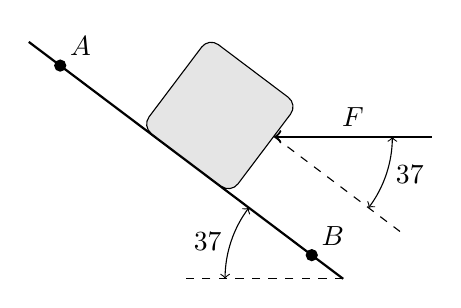
\begin{tikzpicture}
        %% Surface
        \draw[dashed] (0,0) -- (-2,0);
        \draw[thick] (0,0) -- ++ (143:5);
        \draw[<->] (180:1.5) arc (180:143:1.5) node[pos=0.5,anchor=east] {\ang{37}};
        %% Labels
        \draw[fill] (143:4.5) circle (2pt) node[anchor=south west] {$A$};
        \draw[fill] (143:0.5) circle (2pt) node[anchor=south west] {$B$};
        %% Block
        \node[draw,fill=white!90!black,rectangle,rounded corners=1ex,minimum size=1.414cm,rotate=-37,anchor=south] (M) at (143:2.5) {};
        %% Vectors
        \draw[thick,<-] (M.east) ++(53:0.2) -- ++(0:2) node[pos=0.5,anchor=south] {$F$};
        \draw[dashed] (M.east) ++(53:0.2) -- ++(-37:2);
        \draw[<->] (M.east) ++(53:0.2) ++(-37:1.5) arc (-37:0:1.5) node[pos=0.5,anchor=west] {\ang{37}};
    \end{tikzpicture}
    \end{center}
    The kinetic energy of the block at $A$ is \SI{10}{\joule} and at $B$ it is \SI{20}{\joule}.
    How much work is done on the block by the force of friction between $A$ and $B$?
    \begin{multicols}{3}
    \begin{choices}
        \wrongchoice{\SI{-58}{\joule}}
        \wrongchoice{\SI{-53}{\joule}}
      \correctchoice{\SI{-68}{\joule}}
        \wrongchoice{\SI{-63}{\joule}}
        \wrongchoice{\SI{-47}{\joule}}
    \end{choices}
    \end{multicols}
\end{question}
}

\element{serway-mc}{
\begin{question}{serway-ch07-q14}
    If the resultant force acting on a \SI{2.0}{\kilo\gram}
        object is equal to $(3\hat{\imath}+4\hat{\jmath})\,\si{\newton}$,
    what is the change in kinetic energy as the object moves from
        $\left(7\hat{\imath}-8\hat{\jmath}\right)\,\si{\meter}$ to
        $\left(11\hat{\imath}-5\hat{\jmath}\right)\,\si{\meter}$?
    \begin{multicols}{3}
    \begin{choices}
        \wrongchoice{\SI{+36}{\joule}}
        \wrongchoice{\SI{+28}{\joule}}
        \wrongchoice{\SI{+32}{\joule}}
      \correctchoice{\SI{+24}{\joule}}
        \wrongchoice{\SI{+60}{\joule}}
    \end{choices}
    \end{multicols}
\end{question}
}

\element{serway-mc}{
\begin{question}{serway-ch07-q15}
    As a \SI{2.0}{\kilo\gram} object moves from $(2\hat{\imath}+5\hat{\jmath})\,\si{\meter}$ to $(6\hat{\imath}-2\hat{\jmath})\,\si{\meter}$,
        the constant resultant force acting on it is equal to $(4\hat{\imath}-3\hat{\jmath})\,\si{\newton}$.
    If the speed of the object at the initial position is \SI{4.0}{\meter\per\second},
        what is its kinetic energy at its final position?
    \begin{multicols}{3}
    \begin{choices}
        \wrongchoice{\SI{62}{\joule}}
      \correctchoice{\SI{53}{\joule}}
        \wrongchoice{\SI{73}{\joule}}
        \wrongchoice{\SI{86}{\joule}}
        \wrongchoice{\SI{24}{\joule}}
    \end{choices}
    \end{multicols}
\end{question}
}

\element{serway-mc}{
\begin{question}{serway-ch07-q16}
    A block slides on a rough horizontal surface from point $A$ to point $B$. 
    A force (magnitude $P=\SI{2.0}{\newton}$) acts on the block between $A$ and $B$,
        as shown. 
    \begin{center}
    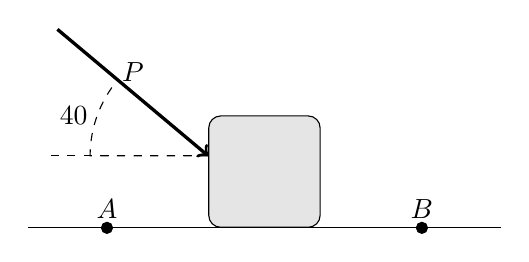
\begin{tikzpicture}
        %% Floor
        \draw (-3,0) -- (3,0);
        \draw[fill] (-2,0) circle (2pt) node[anchor=south] {$A$};
        \draw[fill] (+2,0) circle (2pt) node[anchor=south] {$B$};
        %% Mass
        \node[draw,fill=white!90!black,rectangle,rounded corners=1ex,minimum size=1.414cm,anchor=south] (A) at (0,0) {};
        %% Force
        \draw[dashed] (A.west) ++(90:0.2) -- ++(180:2);
        \draw[dashed] (A.west) ++(90:0.2) -- ++(180:1.5) arc(180:140:1.5) node[pos=0.5,anchor=east] {\ang{40}};
        \draw[very thick,<-] (A.west) ++(90:0.2) -- ++(140:2.5) node[pos=0.5,anchor=south] {$P$};
    \end{tikzpicture}
    \end{center}
    Points $A$ and $B$ are \SI{1.5}{\meter} apart. 
    If the kinetic energies of the block at $A$ and $B$
        are \SI{5.0}{\joule} and \SI{4.0}{\joule}, respectively,
        how much work is done on the block by the force of
        friction as the block moves from $A$ to $B$?
    \begin{multicols}{3}
    \begin{choices}
      \correctchoice{\SI{-3.3}{\joule}}
        \wrongchoice{\SI{+1.3}{\joule}}
        \wrongchoice{\SI{+3.3}{\joule}}
        \wrongchoice{\SI{-1.3}{\joule}}
        \wrongchoice{\SI{+4.6}{\joule}}
    \end{choices}
    \end{multicols}
\end{question}
}

\element{serway-mc}{
\begin{question}{serway-ch07-q17}
    A \SI{2.0}{\kilo\gram} block slides down a frictionless incline from point $A$ to point $B$. 
    A force (magnitude $P=\SI{3.0}{\newton}$) acts on the block between $A$ and $B$,
        as shown. 
    \begin{center}
    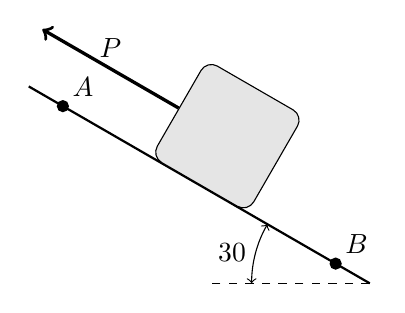
\begin{tikzpicture}
        %% Surface
        \draw[dashed] (0,0) -- (-2,0);
        \draw[thick] (0,0) -- ++ (150:5);
        \draw[<->] (180:1.5) arc (180:150:1.5) node[pos=0.5,anchor=east] {\ang{30}};
        %% Labels
        \draw[fill] (150:4.5) circle (2pt) node[anchor=south west] {$A$};
        \draw[fill] (150:0.5) circle (2pt) node[anchor=south west] {$B$};
        %% Block
        \node[draw,fill=white!90!black,rectangle,rounded corners=1ex,minimum size=1.414cm,rotate=-30,anchor=south] (M) at (150:2.5) {};
        %% Vectors
        \draw[very thick,->] (M.west) -- ++(150:2) node[pos=0.5,anchor=south] {$P$};
    \end{tikzpicture}
    \end{center}
    Points $A$ and $B$ are \SI{2.0}{\meter} apart. 
    If the kinetic energy of the block at $A$ is \SI{10}{\joule},
    what is the kinetic energy of the block at $B$?
    \begin{multicols}{3}
    \begin{choices}
        \wrongchoice{\SI{27}{\joule}}
        \wrongchoice{\SI{20}{\joule}}
      \correctchoice{\SI{24}{\joule}}
        \wrongchoice{\SI{17}{\joule}}
        \wrongchoice{\SI{37}{\joule}}
    \end{choices}
    \end{multicols}
\end{question}
}

\element{serway-mc}{
\begin{question}{serway-ch07-q18}
    A \SI{3.0}{\kilo\gram} block is dragged over a rough horizontal surface by a constant force of \SI{16}{\newton} acting at an angle of \ang{37} above the horizontal as shown. 
    \begin{center}
    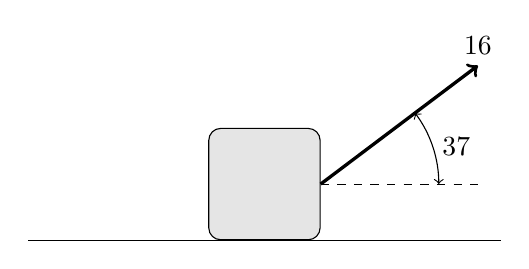
\begin{tikzpicture}
        %% Floor
        \draw (-3,0) -- (3,0);
        %% Mass
        \node[draw,fill=white!90!black,rectangle,rounded corners=1ex,minimum size=1.414cm,anchor=south] (A) at (0,0) {};
        %% Force
        \draw[dashed] (A.east) -- ++(0:2);
        \draw[<->] (A.east) ++(0:1.5) arc(0:37:1.5) node[pos=0.5,anchor=west] {\ang{37}};
        \draw[very thick,->] (A.east) -- ++(37:2.5) node[pos=1.0,anchor=south] {\SI{16}{\newton}};
    \end{tikzpicture}
    \end{center}
    The speed of the block increases from \SI{4.0}{\meter\per\second} to \SI{6.0}{\meter\per\second} in a displacement of \SI{5.0}{\meter}.
    What work was done by the friction force during this displacement?
    \begin{multicols}{3}
    \begin{choices}
      \correctchoice{\SI{-34}{\joule}}
        \wrongchoice{\SI{-64}{\joule}}
        \wrongchoice{\SI{-30}{\joule}}
        \wrongchoice{\SI{-94}{\joule}}
        \wrongchoice{\SI{+64}{\joule}}
    \end{choices}
    \end{multicols}
\end{question}
}

\element{serway-mc}{
\begin{question}{serway-ch07-q19}
    A \SI{6.0}{\kilo\gram} block slides along a horizontal surface. 
    If $\mu_k=\num{0.20}$ for the block and surface,
        at what rate is the friction force doing work on the block at an instant when its speed is \SI{4.0}{\meter\per\second}?
    \begin{multicols}{3}
    \begin{choices}
        \wrongchoice{\SI{-59}{\watt}}
      \correctchoice{\SI{-47}{\watt}}
        \wrongchoice{\SI{-71}{\watt}}
        \wrongchoice{\SI{-82}{\watt}}
        \wrongchoice{\SI{+71}{\watt}}
    \end{choices}
    \end{multicols}
\end{question}
}

\element{serway-mc}{
\begin{question}{serway-ch07-q20}
    At what rate is the gravitational force on a \SI{2.0}{\kilo\gram}
        projectile doing work at an instant when the velocity
        of the projectile is \SI{4.0}{\meter\per\second} directed
        \ang{30} above the horizontal?
    \begin{multicols}{3}
    \begin{choices}
        \wrongchoice{\SI{+39}{\watt}}
        \wrongchoice{\SI{-78}{\watt}}
      \correctchoice{\SI{-39}{\watt}}
        \wrongchoice{\SI{+78}{\watt}}
        \wrongchoice{\SI{+25}{\watt}}
    \end{choices}
    \end{multicols}
\end{question}
}

\element{serway-mc}{
\begin{question}{serway-ch07-q21}
    A \SI{2.0}{\kilo\gram} block slides down a plane (inclined at \ang{40} with the horizontal) at a constant speed of \SI{5.0}{\meter\per\second}. 
    At what rate is the gravitational force on the block doing work?
    \begin{multicols}{3}
    \begin{choices}
        \wrongchoice{\SI{+98}{\watt}}
      \correctchoice{\SI{+63}{\watt}}
        \wrongchoice{zero}
        \wrongchoice{\SI{+75}{\watt}}
        \wrongchoice{\SI{-75}{\watt}}
    \end{choices}
    \end{multicols}
\end{question}
}

\element{serway-mc}{
\begin{question}{serway-ch07-q22}
    The speed of a \SI{4.0}{\kilo\gram} object is given by $v=(2t)\,\si{\meter\per\second}$,
        where $t$ is in seconds.
    At what rate is the resultant force on this object doing work at $t=\SI{1}{\second}$?
    \begin{multicols}{3}
    \begin{choices}
        \wrongchoice{\SI{48}{\watt}}
        \wrongchoice{\SI{40}{\watt}}
        \wrongchoice{\SI{32}{\watt}}
        \wrongchoice{\SI{56}{\watt}}
      \correctchoice{\SI{16}{\watt}}
    \end{choices}
    \end{multicols}
\end{question}
}

\element{serway-mc}{
\begin{question}{serway-ch07-q23}
    A \SI{3.0}{\kilo\gram} block is on a frictionless horizontal surface.
    The block is at rest when,
        at $t=0$, a force (magnitude $P=\SI{2.0}{\newton}$) acting at an angle of \ang{22} above the horizontal is applied to the block.
    At what rate is the force $P$ doing work at $t=\SI{2.0}{\second}$?
    \begin{multicols}{3}
    \begin{choices}
      \correctchoice{\SI{2.3}{\watt}}
        \wrongchoice{\SI{2.0}{\watt}}
        \wrongchoice{\SI{1.4}{\watt}}
        \wrongchoice{\SI{1.7}{\watt}}
        \wrongchoice{\SI{1.2}{\watt}}
    \end{choices}
    \end{multicols}
\end{question}
}

\element{serway-mc}{
\begin{question}{serway-ch07-q24}
    A \SI{1.6}{\kilo\gram} block slides down a plane (inclined at \ang{25} with the horizontal) at a constant speed of \SI{2.0}{\meter\per\second}. 
    At what rate is the frictional force doing work on the block?
    \begin{multicols}{3}
    \begin{choices}
        \wrongchoice{\SI{+28}{\watt}}
        \wrongchoice{\SI{+13}{\watt}}
      \correctchoice{\SI{-13}{\watt}}
        \wrongchoice{\SI{-28}{\watt}}
        \wrongchoice{\SI{+6.5}{\watt}}
    \end{choices}
    \end{multicols}
\end{question}
}

\element{serway-mc}{
\begin{question}{serway-ch07-q25}
    A \SI{3.0}{\kilo\gram} block is on a horizontal surface. 
    The block is at rest when, at $t=0$,
        a force (magnitude $P=\SI{12}{\newton}$) acting parallel to the surface is applied to the block causing it to accelerate. 
        The coefficient of kinetic friction between the block and the surface is \num{0.20}. 
    At what rate is the force $P$ doing work on the block at $t=\SI{2.0}{\second}$?
    \begin{multicols}{3}
    \begin{choices}
        \wrongchoice{\SI{54}{\watt}}
      \correctchoice{\SI{49}{\watt}}
        \wrongchoice{\SI{44}{\watt}}
        \wrongchoice{\SI{59}{\watt}}
        \wrongchoice{\SI{24}{\watt}}
    \end{choices}
    \end{multicols}
\end{question}
}

\element{serway-mc}{
\begin{question}{serway-ch07-q26}
    Starting from rest at $t=0$, a \SI{5.0}{\kilo\gram} block is pulled across a horizontal surface by a constant horizontal force having a magnitude of \SI{12}{\newton}. 
    If the coefficient of friction between the block and the surface is \num{0.20},
        at what rate is the \SI{12}{\newton} force doing work at $t=\SI{5.0}{\second}$?
    \begin{multicols}{3}
    \begin{choices}
        \wrongchoice{\SI{0.13}{\kilo\watt}}
        \wrongchoice{\SI{0.14}{\kilo\watt}}
        \wrongchoice{\SI{0.12}{\kilo\watt}}
      \correctchoice{\SI{26}{\watt}}
        \wrongchoice{\SI{12}{\watt}}
    \end{choices}
    \end{multicols}
\end{question}
}

\element{serway-mc}{
\begin{question}{serway-ch07-q27}
    A \SI{10}{\kilo\gram} block on a horizontal frictionless surface is attached to a light spring (force constant = \SI{0.80}{\kilo\newton\per\meter}). 
    The block is initially at rest at its equilibrium position when a force (magnitude $P=\SI{80}{\newton}$) acting parallel to the surface is applied to the block, as shown. 
    \begin{center}
    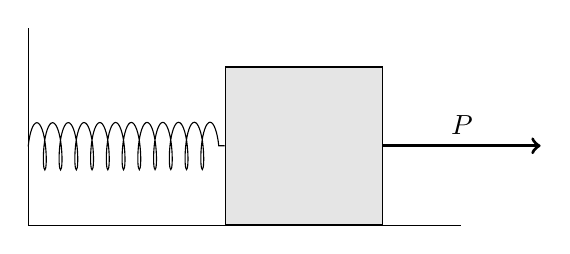
\begin{tikzpicture}
        %% spring/.style = {decorate,decoration={aspect=0.5,segment length=#1,ampltidue=2mm,coil}
        %% playform/.style = {fill,pattern=north east lines,minimum width=2cm,minimum height=0.3cm}
        \draw (0,2.5) -- (0,0) -- (5.5,0);
        \node[fill=white!90!black,draw,rectangle,minimum size=2cm,anchor=south] (M) at (3.5,0) {};
        \draw[decoration={aspect=0.2,segment length=2.0mm,amplitude=3mm,coil},decorate] (0,1) -- (M.west);
        \draw[very thick,->] (M.east) -- +(0:2) node[pos=0.5,anchor=south] {$P$};
    \end{tikzpicture}
    \end{center}
    What is the speed of the block when it is \SI{13}{\centi\meter} from its equilibrium position?
    \begin{multicols}{3}
    \begin{choices}
      \correctchoice{\SI{0.85}{\meter\per\second}}
        \wrongchoice{\SI{0.89}{\meter\per\second}}
        \wrongchoice{\SI{0.77}{\meter\per\second}}
        \wrongchoice{\SI{0.64}{\meter\per\second}}
        \wrongchoice{\SI{0.52}{\meter\per\second}}
    \end{choices}
    \end{multicols}
\end{question}
}

\element{serway-mc}{
\begin{question}{serway-ch07-q28}
    A \SI{10}{\kilo\gram} block on a horizontal frictionless surface is attached to a light spring (force constant = \SI{1.2}{\kilo\newton\per\meter}).
    The block is initially at rest at its equilibrium position when a force (magnitude $P$) acting parallel to the surface is applied to the block,
        as shown. 
    \begin{center}
    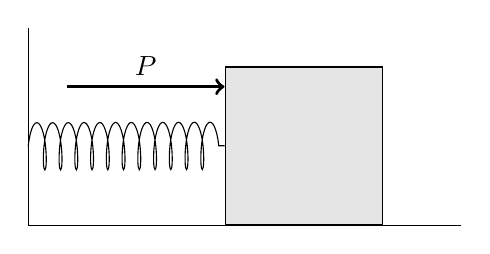
\begin{tikzpicture}
        \draw (0,2.5) -- (0,0) -- (5.5,0);
        \node[fill=white!90!black,draw,rectangle,minimum size=2cm,anchor=south] (M) at (3.5,0) {};
        \draw[decoration={aspect=0.2,segment length=2.0mm,amplitude=3mm,coil},decorate] (0,1) -- (M.west);
        \draw[very thick,<-] (M.west) ++ (90:0.75) -- +(180:2) node[pos=0.5,anchor=south] {$P$};
    \end{tikzpicture}
    \end{center}
    When the block is \SI{8.0}{\centi\meter} from the equilibrium position,
        it has a speed of \SI{0.80}{\meter\per\second}. 
    How much work is done on the block by the force $P$ as the block moves the \SI{8.0}{\centi\meter}?
    \begin{multicols}{3}
    \begin{choices}
        \wrongchoice{\SI{8.3}{\joule}}
        \wrongchoice{\SI{6.4}{\joule}}
      \correctchoice{\SI{7.0}{\joule}}
        \wrongchoice{\SI{7.7}{\joule}}
        \wrongchoice{\SI{3.9}{\joule}}
    \end{choices}
    \end{multicols}
\end{question}
}

\element{serway-mc}{
\begin{question}{serway-ch07-q29}
    A \SI{20}{\kilo\gram} block on a horizontal surface is attached to a light spring (force constant = \SI{8.0}{\kilo\newton\per\meter}). 
    The block is pulled \SI{10}{\centi\meter} to the right from its equilibrium position and released from rest. 
    When the block has moved \SI{2.0}{\centi\meter} toward its equilibrium position, its kinetic energy is \SI{13}{\joule}. 
    How much work is done by the frictional force on the block as it moves the \SI{2.0}{\centi\meter}?
    \begin{multicols}{3}
    \begin{choices}
        \wrongchoice{\SI{-2.5}{\joule}}
      \correctchoice{\SI{-1.4}{\joule}}
        \wrongchoice{\SI{-3.0}{\joule}}
        \wrongchoice{\SI{-1.9}{\joule}}
        \wrongchoice{\SI{-14}{\joule}}
    \end{choices}
    \end{multicols}
\end{question}
}

\element{serway-mc}{
\begin{question}{serway-ch07-q30}
    The horizontal surface on which the block slides is frictionless. 
    The speed of the block before it touches the spring is \SI{6.0}{\meter\per\second}.
    \begin{center}
    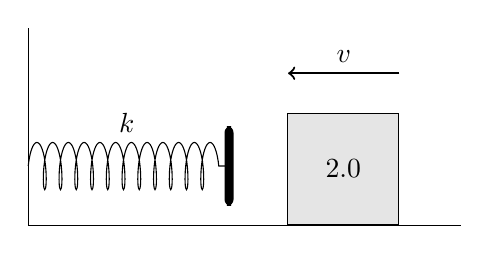
\begin{tikzpicture}
        \draw (0,2.5) -- (0,0) -- (5.5,0);
        \node[fill=white!90!black,draw,rectangle,minimum size=1.414cm,anchor=south] (M) at (4,0) {\SI{2.0}{\kilo\gram}};
        \draw[thick,->] (M.north east) ++ (90:0.5) -- ++ (180:1.414) node[pos=0.5,anchor=south] {$v$};
        \draw[decoration={aspect=0.2,segment length=2.0mm,amplitude=3mm,coil},decorate] (0,0.75) -- (2.5,0.75) node[pos=0.5,anchor=south,yshift=3mm] {$k$};
        \draw[fill=white!50!black,black,rounded corners=0.5ex] (2.5,0.25) rectangle (2.6,1.25);
    \end{tikzpicture}
    \end{center}
    How fast is the block moving at the instant the spring has been compressed \SI{15}{\centi\meter}? 
    $k = \SI{2.0}{\kilo\newton\per\meter}$
    \begin{multicols}{3}
    \begin{choices}
      \correctchoice{\SI{3.7}{\meter\per\second}}
        \wrongchoice{\SI{4.4}{\meter\per\second}}
        \wrongchoice{\SI{4.9}{\meter\per\second}}
        \wrongchoice{\SI{5.4}{\meter\per\second}}
        \wrongchoice{\SI{14}{\meter\per\second}}
    \end{choices}
    \end{multicols}
\end{question}
}

\element{serway-mc}{
\begin{question}{serway-ch07-q31}
    A \SI{2.0}{\kilo\gram} block situated on a frictionless incline is connected to a light spring ($k=\SI{100}{\newton\per\meter}$),
        as shown. 
    The block is released from rest when the spring is unstretched. 
    The pulley is frictionless and has negligible mass. 
    \begin{center}
    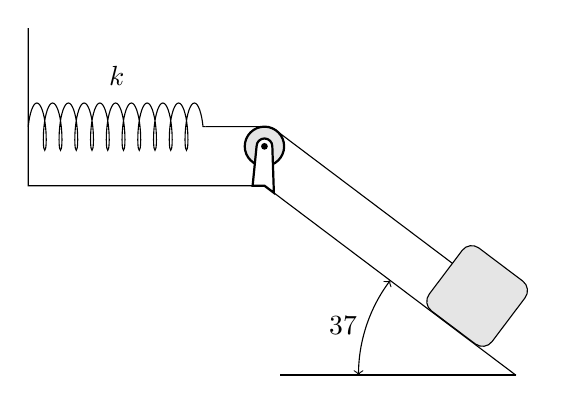
\begin{tikzpicture}
        %% Surface
        \draw (-3,2) -- (-3,0) -- (0,0) -- (323:4);
        \draw[thick] (323:4) -- ++ (180:3);
        \draw[<->] (323:4) ++ (180:2) arc (180:143:2) node[pos=0.5,anchor=east] {\ang{37}};
        %% Blocks
        \node[draw,fill=white!90!black,rectangle,rounded corners=1ex,minimum size=1.00cm,rotate=-37,anchor=south] (M) at (323:3) {};
        %% Spring, Rope
        \draw[decoration={aspect=0.2,segment length=2.0mm,amplitude=3mm,coil},decorate] (-3,0.75) -- (-0.75,0.75) node[pos=0.5,anchor=south,yshift=4mm] {$k$};
        \draw (-0.75,0.75) -- (0,0.75) arc (90:53:0.25) -- ++(323:2.8);
        %% Pulley
        \draw[thick,fill=white!90!black] (0,0.5) circle (0.25); 
        \draw[thick,fill=white] (-0.15,0) -- (-0.1,0.50) arc (180:0:0.1) -- (323:0.15) -- (0,0) -- cycle;
        \draw[fill] (0,0.5) circle (1pt);
    \end{tikzpicture}
    \end{center}
    What is the speed of the block when it has moved \SI{0.20}{\meter} down the plane?
    \begin{multicols}{3}
    \begin{choices}
        \wrongchoice{\SI{76}{\centi\meter\per\second}}
        \wrongchoice{\SI{68}{\centi\meter\per\second}}
      \correctchoice{\SI{60}{\centi\meter\per\second}}
        \wrongchoice{\SI{82}{\centi\meter\per\second}}
        \wrongchoice{\SI{57}{\centi\meter\per\second}}
    \end{choices}
    \end{multicols}
\end{question}
}

\element{serway-mc}{
\begin{question}{serway-ch07-q32}
    A \SI{2.0}{\kilo\gram} block sliding on a frictionless horizontal surface is attached to one end of a horizontal spring ($k=\SI{600}{\newton\per\meter}$) which has its other end fixed. 
    The speed of the block when the spring is extended \SI{20}{\centi\meter} is equal to \SI{3.0}{\meter\per\second}.
    What is the maximum speed of this block as it oscillates?
    \begin{multicols}{3}
    \begin{choices}
      \correctchoice{\SI{4.6}{\meter\per\second}}
        \wrongchoice{\SI{5.3}{\meter\per\second}}
        \wrongchoice{\SI{5.7}{\meter\per\second}}
        \wrongchoice{\SI{4.9}{\meter\per\second}}
        \wrongchoice{\SI{3.5}{\meter\per\second}}
    \end{choices}
    \end{multicols}
\end{question}
}

\element{serway-mc}{
\begin{question}{serway-ch07-q33}
    A \SI{10}{\kilo\gram} block on a rough horizontal surface is attached to a light spring (force constant = \SI{1.4}{\kilo\newton\per\meter}).
    The block is pulled \SI{8.0}{\centi\meter} to the right from its equilibrium position and released from rest. 
    The frictional force between the block and surface has a magnitude of \SI{30}{\newton}. 
    What is the kinetic energy of the block as it passes through its equilibrium position?
    \begin{multicols}{3}
    \begin{choices}
        \wrongchoice{\SI{4.5}{\joule}}
      \correctchoice{\SI{2.1}{\joule}}
        \wrongchoice{\SI{6.9}{\joule}}
        \wrongchoice{\SI{6.6}{\joule}}
        \wrongchoice{\SI{4.9}{\joule}}
    \end{choices}
    \end{multicols}
\end{question}
}

\element{serway-mc}{
\begin{question}{serway-ch07-q34}
    A \SI{2.0}{\kilo\gram} body moving along the $x$ axis has a velocity $v_x=\SI{5.0}{\meter\per\second}$ at $x=0$. 
    The only force acting on the object is given by $F_x=(-4.0x)\,\si{\newton}$,
        where $x$ is in meters. 
    For what value of $x$ will this object first come (momentarily) to rest?
    \begin{multicols}{3}
    \begin{choices}
        \wrongchoice{\SI{4.2}{\meter}}
      \correctchoice{\SI{3.5}{\meter}}
        \wrongchoice{\SI{5.3}{\meter}}
        \wrongchoice{\SI{6.4}{\meter}}
        \wrongchoice{\SI{5.0}{\meter}}
    \end{choices}
    \end{multicols}
\end{question}
}

\element{serway-mc}{
\begin{question}{serway-ch07-q35}
    A \SI{1.5}{\kilo\gram} object moving along the $x$ axis has a velocity of \SI{+4.0}{\meter\per\second} at $x=0$. 
    If the only force acting on this object is shown in the figure,
    \begin{center}
    \begin{tikzpicture}
        \begin{axis}[
            axis y line=left,
            axis x line=middle,
            axis line style={->},
            xlabel={$x$},
            x unit=\si{\meter},
            xtick={0,1,2,3,4},
            ylabel={$F_x$},
            y unit=\si{\newton},
            ytick={-8,-4,0,4,8},
            grid=major,
            xmin=0,xmax=4.5,
            ymin=-5,ymax=9,
            width=0.95\columnwidth,
            height=0.50\columnwidth,
        ]
        \addplot[line width=1pt,mark=\empty] coordinates { (0,8) (3,-4) (5,-4) };
        \end{axis}
    \end{tikzpicture}
    \end{center}
        what is the kinetic energy of the object at $x=\SI{+3.0}{\meter}$?
    \begin{multicols}{3}
    \begin{choices}
      \correctchoice{\SI{18}{\joule}}
        \wrongchoice{\SI{21}{\joule}}
        \wrongchoice{\SI{23}{\joule}}
        \wrongchoice{\SI{26}{\joule}}
        \wrongchoice{\SI{8}{\joule}}
    \end{choices}
    \end{multicols}
\end{question}
}

\element{serway-mc}{
\begin{question}{serway-ch07-q36}
    The only force acting on a \SI{1.6}{\kilo\gram} body as it moves along the $x$ axis is given in the figure. 
    \begin{center}
    \begin{tikzpicture}
        \begin{axis}[
            axis y line=left,
            axis x line=middle,
            axis line style={->},
            xlabel={$x$},
            x unit=\si{\meter},
            xtick={0,2,4,6,8},
            ylabel={$F_x$},
            y unit=\si{\newton},
            ytick={-8,-4,0,4,8},
            grid=major,
            xmin=0,xmax=9,
            ymin=-9,ymax=9,
            width=0.95\columnwidth,
            height=0.50\columnwidth,
        ]
        \addplot[line width=1pt,mark=\empty] coordinates { (0,-8) (4,8) (9,8) };
        \end{axis}
    \end{tikzpicture}
    \end{center}
    If the velocity of the body at $x=\SI{2.0}{\meter}$ is $\SI{5.0}{\meter\per\second}$,
        what is its kinetic energy at $x=\SI{5.0}{\meter}$?
    \begin{multicols}{3}
    \begin{choices}
        \wrongchoice{\SI{52}{\joule}}
        \wrongchoice{\SI{44}{\joule}}
      \correctchoice{\SI{36}{\joule}}
        \wrongchoice{\SI{60}{\joule}}
        \wrongchoice{\SI{25}{\joule}}
    \end{choices}
    \end{multicols}
\end{question}
}

\element{serway-mc}{
\begin{question}{serway-ch07-q37}
    The only force acting on a \SI{2.0}{\kilo\gram} body moving along the $x$ axis is given by $F_x=(2.0x)\,\si{\newton}$,
        where $x$ is in meters. 
    If the velocity of the object at $x=0$ is \SI{+3.0}{\meter\per\second},
        how fast is it moving at $x=\SI{2.0}{\meter}$?
    \begin{multicols}{3}
    \begin{choices}
        \wrongchoice{\SI{4.2}{\meter\per\second}}
      \correctchoice{\SI{3.6}{\meter\per\second}}
        \wrongchoice{\SI{5.0}{\meter\per\second}}
        \wrongchoice{\SI{5.8}{\meter\per\second}}
        \wrongchoice{\SI{2.8}{\meter\per\second}}
    \end{choices}
    \end{multicols}
\end{question}
}

\element{serway-mc}{
\begin{question}{serway-ch07-q38}
    The only force acting on a \SI{2.0}{\kilo\gram} body as it moves along the $x$ axis is given by $F_x=(12-2.0x)\,\si{\newton}$,
        where $x$ is in meters.
    The velocity of the body at $x=\SI{2.0}{\meter}$ is $5.5\hat{\imath}\,\si{\meter\per\second}$.
    What is the maximum kinetic energy attained by the body?
    \begin{multicols}{3}
    \begin{choices}
        \wrongchoice{\SI{36}{\joule}}
        \wrongchoice{\SI{39}{\joule}}
        \wrongchoice{\SI{43}{\joule}}
      \correctchoice{\SI{46}{\joule}}
        \wrongchoice{\SI{30}{\joule}}
    \end{choices}
    \end{multicols}
\end{question}
}

\element{serway-mc}{
\begin{question}{serway-ch07-q39}
    The only force acting on a \SI{1.8}{\kilo\gram} body as it moves along the $x$ axis is given by $F_x=-(3.0x)\,\si{\newton}$,
        where $x$ is in meters.
    If the velocity of the body at $x=0$ is $v_x=\SI{+8.0}{\meter\per\second}$,
        at what value of $x$ will the body have a velocity of \SI{+4.0}{\meter\per\second}?
    \begin{multicols}{3}
    \begin{choices}
        \wrongchoice{\SI{5.7}{\meter}}
      \correctchoice{\SI{5.4}{\meter}}
        \wrongchoice{\SI{4.8}{\meter}}
        \wrongchoice{\SI{4.1}{\meter}}
        \wrongchoice{\SI{6.6}{\meter}}
    \end{choices}
    \end{multicols}
\end{question}
}

\element{serway-mc}{
\begin{question}{serway-ch07-q40}
    Two vectors $\vec{\mathbf{A}}$ and $\vec{\mathbf{B}}$ are given by $\vec{\mathbf{A}}=5\hat{\imath}+6\hat{\jmath}+7\hat{k}$ and $\vec{\mathbf{B}}=3\hat{\imath}-8\hat{\jmath}+2\hat{k}$.
    If these two vectors are drawn starting at the same point,
        what is the angle between them?
    \begin{multicols}{3}
    \begin{choices}
        \wrongchoice{\ang{106}}
      \correctchoice{\ang{102}}
        \wrongchoice{\ang{110}}
        \wrongchoice{\ang{113}}
        \wrongchoice{\ang{97}}
    \end{choices}
    \end{multicols}
\end{question}
}

\element{serway-mc}{
\begin{question}{serway-ch07-q41}
    If $\vec{\mathbf{A}}=7\hat{\imath}-6\hat{\jmath}+5\hat{k}$, $|\vec{\mathbf{B}}|=7$,
        and the angle between $\vec{\mathbf{A}}$ and $\vec{\mathbf{B}}$
        (when the two are drawn starting from the same point) is \ang{60},
        what is the scalar product of these two vectors?
    \begin{multicols}{3}
    \begin{choices}
        \wrongchoice{\num{-13}}
        \wrongchoice{\num{+13}}
      \correctchoice{\num{+37}}
        \wrongchoice{\num{-37}}
        \wrongchoice{\num{73}}
    \end{choices}
    \end{multicols}
\end{question}
}

\element{serway-mc}{
\begin{question}{serway-ch07-q42}
    If vectors $\vec{\mathbf{A}}$ and $\vec{\mathbf{B}}$ have magnitudes 12 and 15,
        respectively, and the angle between the two when they are drawn starting from the same point is \ang{110},
        what is the scalar product of these two vectors?
    \begin{multicols}{3}
    \begin{choices}
        \wrongchoice{\num{-76}}
      \correctchoice{\num{-62}}
        \wrongchoice{\num{-90}}
        \wrongchoice{\num{-47}}
        \wrongchoice{\num{-170}}
    \end{choices}
    \end{multicols}
\end{question}
}

\element{serway-mc}{
\begin{question}{serway-ch07-q43}
    If the vectors $\vec{\mathbf{A}}$ and $\vec{\mathbf{B}}$ have magnitudes of 10 and 11,
        respectively, and the scalar product of these two vectors is \num{-100},
        what is the magnitude of the sum of these two vectors?
    \begin{multicols}{3}
    \begin{choices}
        \wrongchoice{\num{6.6}}
      \correctchoice{\num{4.6}}
        \wrongchoice{\num{8.3}}
        \wrongchoice{\num{9.8}}
        \wrongchoice{\num{7.6}}
    \end{choices}
    \end{multicols}
\end{question}
}

\element{serway-mc}{
\begin{question}{serway-ch07-q44}
    If the scalar product of two vectors, $\vec{\mathbf{A}}$ and $\vec{\mathbf{C}}$,
        is equal to \num{-3.5}, if $|\vec{\mathbf{A}}|=2.0$,
        and the angle between the two vectors when they are drawn starting from the same point is equal to \ang{130},
        what is the magnitude of $\vec{\mathbf{C}}$?
    \begin{multicols}{3}
    \begin{choices}
        \wrongchoice{\num{2.1}}
        \wrongchoice{\num{2.5}}
        \wrongchoice{\num{2.3}}
      \correctchoice{\num{2.7}}
        \wrongchoice{\num{3.1}}
    \end{choices}
    \end{multicols}
\end{question}
}

\element{serway-mc}{
\begin{question}{serway-ch07-q45}
    If $\vec{\mathbf{A}}\cdot\vec{\mathbf{C}}=-7.5$, $\vec{\mathbf{A}}=3\hat{\imath}-4\hat{\jmath}$, and $|\vec{\mathbf{C}}|=6.5$,
        what is the angle between the two vectors when they are drawn starting from the same point?
    \begin{multicols}{3}
    \begin{choices}
        \wrongchoice{\ang{118}}
        \wrongchoice{\ang{107}}
        \wrongchoice{\ang{112}}
      \correctchoice{\ang{103}}
        \wrongchoice{\ang{77}}
    \end{choices}
    \end{multicols}
\end{question}
}

\element{serway-mc}{
\begin{question}{serway-ch07-q46}
    Two vectors $\vec{\mathbf{A}}$ and $\vec{\mathbf{B}}$ are given by $\vec{\mathbf{A}}=4\hat{\imath}+8\hat{\jmath}$ and $\vec{\mathbf{B}}=6\hat{\imath}-2\hat{\jmath}$.
    The scalar product of $\vec{\mathbf{A}}$ and a third vector $\vec{\mathbf{C}}$ is \num{-16}.
    The scalar product of $\vec{\mathbf{B}}$ and $\vec{\mathbf{C}}$ is \num{+18}.
    The $z$ component of $\vec{\mathbf{C}}$ is \num{0}.
    What is the magnitude of $\vec{\mathbf{C}}$?
    \begin{multicols}{3}
    \begin{choices}
        \wrongchoice{\num{7.8}}
        \wrongchoice{\num{6.4}}
      \correctchoice{\num{3.6}}
        \wrongchoice{\num{5.0}}
        \wrongchoice{\num{4.8}}
    \end{choices}
    \end{multicols}
\end{question}
}

\element{serway-mc}{
\begin{question}{serway-ch07-q47}
    If $\vec{\mathbf{A}}=10$, $\vec{\mathbf{B}}=15$, and $\alpha =\ang{130}$,
        determine the scalar product of the two vectors shown.
    \begin{center}
    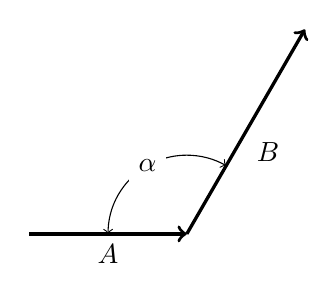
\begin{tikzpicture}
        \draw[very thick,->] (-2,0) -- (0,0) node[anchor=north,pos=0.5] {$A$};
        \draw[very thick,->] (0,0) -- (60:3) node[anchor=north west,pos=0.5] {$B$};
        \draw[<->] (180:1) arc (180:60:1) node[anchor=center,fill=white,pos=0.5] {$\alpha$};
    \end{tikzpicture}
    \end{center}
    \begin{multicols}{3}
    \begin{choices}
      \correctchoice{\num{+96}}
        \wrongchoice{\num{-96}}
        \wrongchoice{\num{+51}}
        \wrongchoice{\num{-51}}
        \wrongchoice{\num{-35}}
    \end{choices}
    \end{multicols}
\end{question}
}

\element{serway-mc}{
\begin{question}{serway-ch07-q48}
    If $\vec{\mathbf{A}}=5.0$, $\vec{\mathbf{B}}=8.0$, and $\alpha=\ang{30}$,
        determine the scalar product of the two vectors shown.
    \begin{center}
    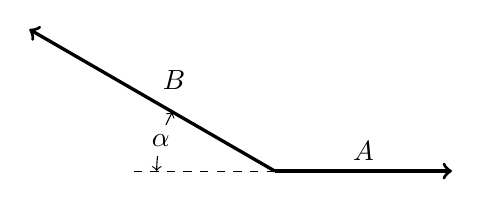
\begin{tikzpicture}[scale=0.75]
        \draw[very thick,->] (0,0) -- (3,0) node[anchor=south,pos=0.5] {$A$};
        \draw[very thick,->] (0,0) -- (150:4.8) node[anchor=south west,pos=0.5] {$B$};
        \draw[dashed] (0,0) -- (-2.5,0);
        \draw[<->] (180:2.0) arc (180:150:2) node[anchor=center,fill=white,pos=0.5] {$\alpha$};
    \end{tikzpicture}
    \end{center}
    \begin{multicols}{3}
    \begin{choices}
      \correctchoice{\num{-35}}
        \wrongchoice{\num{+35}}
        \wrongchoice{\num{-20}}
        \wrongchoice{\num{+20}}
        \wrongchoice{\num{+40}}
    \end{choices}
    \end{multicols}
\end{question}
}

\element{serway-mc}{
\begin{question}{serway-ch07-q49}
    If $\vec{\mathbf{A}}=6.0$, $\vec{\mathbf{B}}=5.0$, and $\alpha=\ang{40}$,
        determine the scalar product of the two vectors shown.
    \begin{center}
    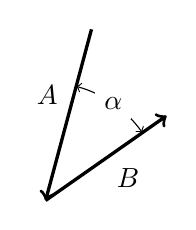
\begin{tikzpicture}[scale=0.75]
        \draw[very thick,<-] (0,0) -- (75:3) node[anchor=south east,pos=0.5] {$A$};
        \draw[very thick,->] (0,0) -- (35:2.5) node[anchor=north west,pos=0.5] {$B$};
        \draw[<->] (75:2) arc (75:35:2) node[anchor=center,fill=white,pos=0.5] {$\alpha$};
    \end{tikzpicture}
    \end{center}
    \begin{multicols}{3}
    \begin{choices}
        \wrongchoice{\num{+19}}
        \wrongchoice{\num{+23}}
        \wrongchoice{\num{-19}}
      \correctchoice{\num{-23}}
        \wrongchoice{\num{+30}}
    \end{choices}
    \end{multicols}
\end{question}
}

\element{serway-mc}{
\begin{question}{serway-ch07-q50}
    The same constant force is used to accelerate two carts of the same mass,
        initially at rest, on horizontal frictionless tracks. 
    The force is applied to cart $A$ for twice as long a time as it is applied to cart $B$. 
    The work the force does on $A$ is $W_A$; that on $B$ is $W_B$. 
    Which statement is correct?
    \begin{multicols}{2}
    \begin{choices}
        \wrongchoice{$W_A = W_B$}
        \wrongchoice{$W_A = \sqrt{2} W_B$}
        \wrongchoice{$W_A = 2 W_B$}
      \correctchoice{$W_A = 4 W_B$}
        \wrongchoice{$W_B = 2 W_A$}
    \end{choices}
    \end{multicols}
\end{question}
}

\element{serway-mc}{
\begin{question}{serway-ch07-q51}
    Carts $A$ and $B$ have equal masses and travel equal distances on straight frictionless tracks while a constant force $F$ is applied to $A$,
        and a constant force $2F$ is applied to $B$. 
    The relative amounts of work done by the two forces are related:
    \begin{multicols}{2}
    \begin{choices}
        \wrongchoice{$W_A = 4 W_B$}
        \wrongchoice{$W_A = 2 W_B$}
        \wrongchoice{$W_A = W_B$}
      \correctchoice{$W_B = 2 W A$}
        \wrongchoice{$W_B = 4 W_A$}
    \end{choices}
    \end{multicols}
\end{question}
}

\element{serway-mc}{
\begin{question}{serway-ch07-q52}
    Carts $A$ and $B$ have equal masses and travel equal distances $D$ on side-by-side straight frictionless tracks while a constant force $F$ acts on $A$ and a constant force $2F$ acts on $B$. 
    Both carts start from rest. 
    The velocities $v_A$ and $v_B$ of the bodies at the end of distance $D$ are related by:
    \begin{multicols}{2}
    \begin{choices}
        \wrongchoice{$v_B = v_A$}
      \correctchoice{$v_B = \sqrt{2} v_A$}
        \wrongchoice{$v_B = 2 v_A$}
        \wrongchoice{$v_B = 4 v_A$}
        \wrongchoice{$v_A = 2 v_B$}
    \end{choices}
    \end{multicols}
\end{question}
}

\element{serway-mc}{
\begin{question}{serway-ch07-q53}
    Two equal masses are raised at constant velocity by ropes that run over pulleys,
        as shown below. 
    \begin{center}
    \begin{tikzpicture}
        %% Ceiling
        \node[anchor=south,fill,pattern=north east lines,minimum width=8cm, minimum height=0.05cm] at (0,0) {};
        \draw (-4,0) -- (4,0);
        %% Pulley A and B
        \draw (-2,-0.5) circle (0.25cm);
        \draw (+2,-0.5) circle (0.25cm);
        \draw[fill=white!60!black] (-2.2,0) -- (-2.1,-0.55) arc(190:350:0.1cm) -- (-1.8,0) -- cycle;
        \draw[fill=white!60!black] (+2.2,0) -- (+2.1,-0.55) arc(350:180:0.1cm) -- (+1.8,0) -- cycle;
        \draw[fill] (-2,-0.5) circle (1pt);
        \draw[fill] (+2,-0.5) circle (1pt);
        %% Mass A and B
        \node[draw,fill=white!90!black,rectangle,rounded corners=1ex,minimum size=1.00cm,anchor=north] (A) at (-1.75,-3.5) {$A$};
        \node[draw,fill=white!90!black,rectangle,rounded corners=1ex,minimum size=1.00cm,anchor=north] (B) at (+1.75,-2.5) {$B$};
        %% Rope
        \draw[thick] (A.north) -- (-1.75,-0.5) arc(0:160:0.25) -- (-3.25,-5.5);
        \draw[thick] (B.north) -- (+1.75,-0.5) arc(180:20:0.25) -- (+3.25,-5.5);
        %% Machine Housing
        \draw[rounded corners=2pt] (-3.4,-6) rectangle (-2.6,-5.5);
        \draw[rounded corners=2pt] (+3.4,-6) rectangle (+2.6,-5.5);
        \draw[fill,rounded corners=2pt] (-3.5,-6) rectangle (-2.5,-5.9);
        \draw[fill,rounded corners=2pt] (+3.5,-6) rectangle (+2.5,-5.9);
        %% Machines Pulley
        \draw[fill=white!90!black] (-3,-5.5) circle (0.25cm);
        \draw[fill=white!90!black] (+3,-5.5) circle (0.25cm);
        \draw (-3,-5.5) circle (0.12cm);
        \draw (+3,-5.5) circle (0.12cm);
        \draw (-2.2,0) -- (-2.1,-0.55) arc(190:350:0.1cm) -- (-1.8,0) -- cycle;
        \draw (+2.2,0) -- (+2.1,-0.55) arc(350:180:0.1cm) -- (+1.8,0) -- cycle;
        \draw[fill] (-2,-0.5) circle (1pt);
        \draw[fill] (+2,-0.5) circle (1pt);
        %% Floor
        \draw (-4,-6) -- (4,-6);
        \node[anchor=north,fill,pattern=north east lines,minimum width=8cm, minimum height=0.05cm] at (0,-6) {};
    \end{tikzpicture}
    \end{center}
    Mass $B$ is raised twice as fast as mass $A$. 
    The magnitudes of the forces are $F_A$ and $F_B$,
        while the power supplied is respectively $P_A$ and $P_B$. 
    Which statement is correct?
    \begin{choices}
        \wrongchoice{$F_B = F_A$;    $P_B = P_A$}
      \correctchoice{$F_B = F_A$;    $P_B = 2 P_A$}
        \wrongchoice{$F_B = 2 F_A$;  $P_B = P_A$}
        \wrongchoice{$F_B = 2 F_A$;  $P_B = 2 P_A$}
        \wrongchoice{$P_A = F_A$;    $P_B = F_B$}
    \end{choices}
\end{question}
}

\element{serway-mc}{
\begin{question}{serway-ch07-q54}
    When a ball rises vertically to a height $h$ and returns to its original point of projection,
        the work done by the gravitational force is:
    \begin{multicols}{3}
    \begin{choices}
      \correctchoice{zero}
        \wrongchoice{$-mgh$}
        \wrongchoice{$+mgh$}
        \wrongchoice{$-2mgh$}
        \wrongchoice{$+2mgh$}
    \end{choices}
    \end{multicols}
\end{question}
}

\element{serway-mc}{
\begin{question}{serway-ch07-q55}
    When a crate of mass $m$ is dragged a distance $d$ along a surface with coefficient of kinetic friction $\mu_k$,
        then dragged back along the same path to its original position,
        the work done by friction is:
    \begin{multicols}{3}
    \begin{choices}
        \wrongchoice{zero}
        \wrongchoice{$-\mu_k mgd$}
        \wrongchoice{$+\mu_k mgd$}
      \correctchoice{$-2\mu_k mgd$}
        \wrongchoice{$+2\mu_k mgd$}
    \end{choices}
    \end{multicols}
\end{question}
}

\element{serway-mc}{
\begin{question}{serway-ch07-q56}
    Two balls, $A$ and $B$, of mass $m$ and $2m$ respectively,
        are carried to height $h$ at constant velocity,
        but $B$ rises twice as fast as $A$.
    The work the gravitational force does on $B$ is:
    \begin{choices}
        \wrongchoice{one quarter the work done on $A$.}
        \wrongchoice{one half the work done on $A$.}
        \wrongchoice{the same as the work done on $A$.}
      \correctchoice{twice the work done on $A$.}
        \wrongchoice{four times the work done on $A$.}
    \end{choices}
\end{question}
}

\element{serway-mc}{
\begin{question}{serway-ch07-q57}
    Equal amounts of work are performed on two bodies, A and B,
        initially at rest, and of masses $M$ and $2M$ respectively. 
    The relation between their speeds immediately after
        the work has been done on them is:
    \begin{multicols}{2}
    \begin{choices}
      \correctchoice{$v_A = \sqrt{2} v_B$}
        \wrongchoice{$v_A = 2 v_B$}
        \wrongchoice{$v_A = v_B$}
        \wrongchoice{$v_B = \sqrt{2} v_A$}
        \wrongchoice{$v_B = 2 v_A$}
    \end{choices}
    \end{multicols}
\end{question}
}

\element{serway-mc}{
\begin{question}{serway-ch07-q58}
    Two cannonballs are dropped from a second floor physics lab at height $h$ above the ground.
    Ball $B$ has four times the mass of ball $A$. 
    When the balls pass the bottom of a first floor window at height $h/4$ above the ground,
        the relation between their kinetic energies, $K_A$ and $K_B$ is:
    \begin{multicols}{2}
    \begin{choices}
        \wrongchoice{$K_A = 4 K_B$}
        \wrongchoice{$K_A = 2 K_B$}
        \wrongchoice{$K_A = K_B$}
        \wrongchoice{$K_B = 2 K_A$}
      \correctchoice{$K_B = 4 K_A$}
    \end{choices}
    \end{multicols}
\end{question}
}

\element{serway-mc}{
\begin{question}{serway-ch07-q59}
    Two clowns are launched from the same spring-loaded circus cannon with the spring compressed the same distance each time. 
    Clown $A$ has a \SI{40}{\kilo\gram} mass; clown $B$ a \SI{60}{\kilo\gram} mass. 
    The relation between their kinetic energies at the instant of launch is:
    \begin{multicols}{2}
    \begin{choices}
        \wrongchoice{$K_A = \dfrac{3}{2} K_B$}
        \wrongchoice{$K_A = \sqrt{\dfrac{3}{2}} K_B$}
      \correctchoice{$K_A = K_B$}
        \wrongchoice{$K_B = \sqrt{\dfrac{3}{2}} K_A$}
        \wrongchoice{$K_B = \sqrt{\dfrac{3}{2}} K_A$}
    \end{choices}
    \end{multicols}
\end{question}
}

\element{serway-mc}{
\begin{question}{serway-ch07-q60}
    Two clowns are launched from the same spring-loaded
        circus cannon with the spring compressed the same distance each time. 
    Clown $A$ has a \SI{40}{\kilo\gram} mass;
        clown $B$ a \SI{60}{\kilo\gram} mass. 
    The relation between their speeds at the instant of launch is:
    \begin{multicols}{2}
    \begin{choices}
        \wrongchoice{$v_A = \dfrac{3}{2} v_B$}
      \correctchoice{$v_A = \sqrt{\dfrac{3}{2}} v_B$}
        \wrongchoice{$v_A = v_B$}
        \wrongchoice{$v_B = \sqrt{\dfrac{3}{2}} v_A$}
        \wrongchoice{$v_B = \dfrac{3}{2} v_A$}
    \end{choices}
    \end{multicols}
\end{question}
}

\element{serway-mc}{
\begin{question}{serway-ch07-q61}
    In a contest, two tractors pull two identical blocks of stone the same distance over identical surfaces.
    However, block $A$ is moving twice as fast as block $B$ when it crosses the finish line. 
    Which statement is correct?
    \begin{choices}
        \wrongchoice{Block $A$ has twice as much kinetic energy as block $B$.}
        \wrongchoice{Block $B$ has lost twice as much kinetic energy to friction as block $A$.}
        \wrongchoice{Block $B$ has lost twice as much kinetic energy as block $A$.}
      \correctchoice{Both blocks have had equal losses of energy to friction.}
        \wrongchoice{No energy is lost to friction because the ground has no displacement.}
    \end{choices}
\end{question}
}

\element{serway-mc}{
\begin{question}{serway-ch07-q62}
    If the scalar (dot) product of two vectors is negative, it means that:
    \begin{choices}
        \wrongchoice{there was a calculator error.}
        \wrongchoice{the angle between the vectors is less than 90 degrees.}
        \wrongchoice{the angle between the vectors is 90 degrees.}
        \wrongchoice{the angle between the vectors is greater than 270 degrees.}
      \correctchoice{the angle between the vectors is between 90 and 180 degrees.}
    \end{choices}
\end{question}
}

\element{serway-mc}{
\begin{question}{serway-ch07-q63}
    Two eggs of equal mass are thrown at a blanket with equal velocity. 
    Egg $B$ hits the blanket but egg $A$ hits the wall instead. 
    Compare the work done on the eggs in reducing their velocities to zero.
    \begin{choices}
        \wrongchoice{More work was done on $A$ than on $B$.}
        \wrongchoice{More work was done on $B$ than on $A$.}
      \correctchoice{The amount of work is the same for both.}
        \wrongchoice{It is meaningless to compare the amount of work because the forces were so different.}
        \wrongchoice{Work was done on $B$, but no work was done on $A$ because the wall did not move.}
    \end{choices}
\end{question}
}

\element{serway-mc}{
\begin{question}{serway-ch07-q64}
    Planets go around the sun in elliptical orbits. 
    The highly exaggerated diagram below shows a portion of such an orbit and the force on the planet at one position along that orbit. 
    \begin{center}
    \begin{tikzpicture}
        \draw[dashed] (0,0) circle (3cm and 2cm);
        \draw[fill=white!90!black] (2.236,1.35) circle (4pt);
        \draw[thick,->] (2.236,1.35) -- ++(197:2) node[pos=0.5,anchor=south east] {$F$};
        \draw[thick,->] (2.236,1.35) -- ++(-42:1) node[pos=0.5,anchor=south west] {$v$};
    \end{tikzpicture}
    \end{center}
    The planet is moving to the right.
    $F_{\parallel}$ and $F_{\perp}$ are the components of the force parallel
        (tangential) and perpendicular (normal) to the orbit. 
    The work they do is $W_{\parallel}$ and $W_{\perp}$. 
    At the position shown:
    \begin{choices}
        \wrongchoice{$W_{\parallel}$ slows the planet down; $W_{\perp}$ speeds it up.}
      \correctchoice{$W_{\parallel}$ slows the planet down; $W_{\perp}$ does no work on it.}
        \wrongchoice{$W_{\parallel}$ speeds the planet up; $W_{\perp}$ does no work on it.}
        \wrongchoice{$W_{\parallel}$ speeds the planet up; $W_{\perp}$ slows it down.}
        \wrongchoice{$W_{\parallel}$ does no work on it; $W_{\perp}$ speeds the planet up.}
    \end{choices}
\end{question}
}

\element{serway-mc}{
\begin{question}{serway-ch07-q65}
    A mass attached to the end of a spring is pulled out and released on a surface with friction. 
    The work $\vec{\mathbf{F}}_{sp}\cdot\mathrm{d}\vec{\mathbf{x}}$ done on the mass by the force exerted by the spring:
    \begin{choices}
        \wrongchoice{never has the same sign as the change in energy owing to friction.}
        \wrongchoice{always has the same sign as the change in energy owing to friction.}
      \correctchoice{has the same sign as the change in energy owing to friction during one half of each cycle.}
        \wrongchoice{never has the same sign as the change in energy owing to friction if the force of friction is greater than the spring force.}
        \wrongchoice{always has the same sign as the change in energy owing to friction if the force of friction is greater than the spring force.}
    \end{choices}
\end{question}
}

\element{serway-mc}{
\begin{question}{serway-ch07-q66}
    The work $\vec{\mathbf{F}}_{sp}\cdot\mathrm{d}\vec{\mathbf{x}}$ done by the force exerted by the spring on a mass attached to the end of the spring when the mass has displacement $\mathrm{d}\vec{\mathbf{x}}$ is:
    \begin{choices}
        \wrongchoice{always negative.}
        \wrongchoice{always positive.}
      \correctchoice{negative half the time, positive the other half of the time.}
        \wrongchoice{positive more than it is negative.}
        \wrongchoice{negative more than it is positive.}
    \end{choices}
\end{question}
}

\element{serway-mc}{
\begin{question}{serway-ch07-q67}
    A \SI{30}{\kilo\gram} child sitting \SI{5.0}{\meter} from the center of a merry-go-round has a constant speed of \SI{5.0}{\meter\per\second}.
    While she remains seated in the same spot and travels in a circle,
        the work the seat performs on her in one complete rotation is:
    \begin{multicols}{2}
    \begin{choices}
      \correctchoice{\SI{0}{\joule}}
        \wrongchoice{\SI{150}{\joule}}
        \wrongchoice{\SI{1500}{\joule}}
        \wrongchoice{\SI{4700}{\joule}}
        \wrongchoice{\SI{46 000}{\joule}}
    \end{choices}
    \end{multicols}
\end{question}
}

\element{serway-mc}{
\begin{question}{serway-ch07-q68}
    Sally, who weighs \SI{450}{\newton},
        stands on a skate board while Roger pushes it forward \SI{13.0}{\meter} at constant velocity on a level straight street.
    He applies a constant \SI{100}{\newton} force.
    \begin{choices}
        \wrongchoice{The work Roger does on the skateboard is \SI{0}{\joule}.}
      \correctchoice{The work Roger does on the skateboard is \SI{1300}{\joule}.}
        \wrongchoice{The work Sally does on the skateboard is \SI{1300}{\joule}.}
        \wrongchoice{The work Sally does on the skateboard is \SI{5850}{\joule}.}
        \wrongchoice{The work Roger does on the skateboard is \SI{5850}{\joule}.}
    \end{choices}
\end{question}
}

\element{serway-mc}{
\begin{question}{serway-ch07-q69}
    After jumping up and down on a diving board,
        Roger jumps off the diving board. 
    Hakim claims that Roger does work on the diving board because he supplies energy to it. 
    Ludmilla claims that the diving board does work on Roger and supplies energy to him. 
    Which one, if either, is correct?
    \begin{choices}
      \correctchoice{Hakim, because the diving board is deformed and vibrated like a spring when Roger jumps.}
        \wrongchoice{Ludmilla, because Roger jumps up in the air above the diving board.}
        \wrongchoice{Neither, because Roger's muscles do all the work.}
        \wrongchoice{Both, because Roger's muscles do all the work.}
        \wrongchoice{Neither, because the diving board does all the work.}
    \end{choices}
\end{question}
}

\element{serway-mc}{
\begin{question}{serway-ch07-q70}
    Negative work can be done:
    \begin{choices}[o]
        \wrongchoice{by friction while a car is accelerating without skidding.}
        \wrongchoice{by a spring at the bottom of an elevator shaft when it stops a falling elevator.}
        \wrongchoice{by a hand catching a ball.}
        \wrongchoice{by all of the above}
      \correctchoice{by only (b) and (c) above}
    \end{choices}
\end{question}
}

\element{serway-mc}{
\begin{question}{serway-ch07-q71}
    Positive work can be done
    \begin{choices}[o]
        \wrongchoice{by friction while a car is accelerating without skidding.}
        \wrongchoice{by a spring at the bottom of an elevator shaft when it stops a falling elevator.}
        \wrongchoice{by a hand throwing a ball.}
        \wrongchoice{by all of the above}
      \correctchoice{by only (b) and (c) above}
    \end{choices}
\end{question}
}

%% NOTE: q70 and q71 alternatives
%\element{serway-mc}{
%\begin{questionmult}{serway-ch07-q70A}
%    Negative work can be done:
%    \begin{choices}
%        \wrongchoice{by a spring when it launches a clown in the air.}
%        \wrongchoice{by a hand throwing a ball.}
%      \correctchoice{by a spring at the bottom of an elevator shaft when it stops a falling elevator.}
%      \correctchoice{by a hand catching a ball.}
%    \end{choices}
%\end{questionmult}
%}
%
%\element{serway-mc}{
%\begin{questionmult}{serway-ch07-q71A}
%    Positive work can be done
%    \begin{choices}
%      \correctchoice{by a spring when it launches a clown in the air.}
%      \correctchoice{by a hand throwing a ball.}
%        \wrongchoice{by a spring at the bottom of an elevator shaft when it stops a falling elevator.}
%        \wrongchoice{by a hand catching a ball.}
%    \end{choices}
%\end{questionmult}
%}

\element{serway-mc}{
\begin{question}{serway-ch07-q72}
    The force of static friction exerted on an automobile's tires by the ground:
    \begin{choices}[o]
      \correctchoice{provides the accelerating force that makes the car move forward.}
        \wrongchoice{does positive work on the car while it is accelerating.}
        \wrongchoice{does negative work on the car while it is decelerating.}
        \wrongchoice{does everything listed in (a), (b) and (c).}
        \wrongchoice{only does positive or negative work as in (b) or (c).}
    \end{choices}
\end{question}
}

\element{serway-mc}{
\begin{question}{serway-ch07-q73}
    The graph below shows how the force on a \SI{0.500}{\kilo\gram} particle varies with position.
    \begin{center}
    \begin{tikzpicture}
        \begin{axis}[
            axis y line=left,
            axis x line=bottom,
            axis line style={->},
            xlabel={position},
            x unit=\si{\meter},
            xtick={0,2,4,6,8,10,12},
            ylabel={force},
            y unit=\si{\newton},
            ytick={0,2,4,6,8,10,12},
            grid=major,
            xmin=0,xmax=12,
            ymin=0,ymax=12,
            width=0.95\columnwidth,
            height=0.50\columnwidth,
        ]
        \addplot[line width=1pt,mark=\empty] coordinates { (0,0) (5,10) (8,10) (10,4) };
        \end{axis}
    \end{tikzpicture}
    \end{center}
    If the particle has speed $v=\SI{2.23}{\meter\per\second}$ at $x=\SI{2.00}{\meter}$,
        what is its speed when $x=\SI{8.00}{\meter}$?
    \begin{multicols}{2}
    \begin{choices}
        \wrongchoice{\SI{2.00}{\meter\per\second}}
        \wrongchoice{\SI{10.7}{\meter\per\second}}
        \wrongchoice{\SI{14.8}{\meter\per\second}}
      \correctchoice{\SI{15.0}{\meter\per\second}}
        \wrongchoice{\SI{21.1}{\meter\per\second}}
    \end{choices}
    \end{multicols}
\end{question}
}

\element{serway-mc}{
\begin{question}{serway-ch07-q74}
    The equation below is the solution to a physics problem:
    \begin{align*}
        &\dfrac{1}{2}\left(\SI{2.30}{\kilo\gram}\right)\left(\SI{5.00}{\meter\per\second}\right)^2 = \\
        &\quad\quad\dfrac{1}{2}\left(\SI{2.30}{\kilo\gram}\right)\left(\SI{2.33}{\meter\per\second}\right)^2 \\
        &\quad\quad+\left(\SI{2.30}{\kilo\gram}\right)\left(\SI{9.80}{\meter\per\second\squared}\right)\left(\SI{1.00}{\meter}\right)\cos(\ang{60}).
    \end{align*}
    The most likely physical situation it describes is:
    \begin{choices}
        \wrongchoice{a \SI{2.30}{\kilo\gram} cart rolling up a \ang{30} incline.}
      \correctchoice{a \SI{2.30}{\kilo\gram} cart rolling down a \ang{30} incline.}
        \wrongchoice{a \SI{2.30}{\kilo\gram} cart rolling up a \ang{60} incline.}
        \wrongchoice{a \SI{2.30}{\kilo\gram} cart rolling down a \ang{60} incline.}
        \wrongchoice{a \SI{2.30}{\kilo\gram} cart rolling down a \ang{90} incline.}
    \end{choices}
\end{question}
}

\element{serway-mc}{
\begin{question}{serway-ch07-q75}
    A compressed spring is used to launch a skier up an icy ski slope with a \ang{20} incline. 
    How far up the incline the skier travels may depend on the following factors.
    To find the distance up the slope we do \emph{not} need to know:
    \begin{choices}
      \correctchoice{the skier's mass.}
        \wrongchoice{how far the spring is compressed.}
        \wrongchoice{the force constant of the spring}
        \wrongchoice{the angle of incline of the slope.}
        \wrongchoice{the value of the gravitational constant $g$ at that location.}
    \end{choices}
\end{question}
}

\element{serway-mc}{
\begin{question}{serway-ch07-q76}
    After a skydiver reaches terminal velocity,
    \begin{choices}
        \wrongchoice{the force of gravity no longer performs work on the skydiver.}
        \wrongchoice{work performed by the force of gravity is converted into gravitational potential energy.}
        \wrongchoice{gravitational potential energy is no longer available to the system of the skydiver plus the Earth.}
      \correctchoice{gravitational potential energy is converted into thermal energy.}
        \wrongchoice{thermal energy is converted into gravitational potential energy.}
    \end{choices}
\end{question}
}


\endinput


